% Generated by figures/_scene.py (Scene.render_tikz) for 'Fig 1 teaser maize 4 to 4'; do not edit by hand, re-run the figure script.
% 6.875 x 2.5 in at 100 %; needs \usetikzlibrary{arrows.meta}; images in Figures/fig1b/.
{%
\definecolor{c1A1A1A}{HTML}{1A1A1A}%
\definecolor{c3F5F8F}{HTML}{3F5F8F}%
\definecolor{c5E4A96}{HTML}{5E4A96}%
\definecolor{c5F5F5F}{HTML}{5F5F5F}%
\definecolor{c809EC2}{HTML}{809EC2}%
\definecolor{c8C8C8C}{HTML}{8C8C8C}%
\definecolor{c9D8CC4}{HTML}{9D8CC4}%
\definecolor{cA07800}{HTML}{A07800}%
\definecolor{cA8456E}{HTML}{A8456E}%
\definecolor{cD091A7}{HTML}{D091A7}%
\definecolor{cE0B020}{HTML}{E0B020}%
\definecolor{cE6ECF3}{HTML}{E6ECF3}%
\definecolor{cEAE7F2}{HTML}{EAE7F2}%
\definecolor{cF6E9ED}{HTML}{F6E9ED}%
\definecolor{cFAF2D4}{HTML}{FAF2D4}%
\begin{tikzpicture}[x=1in, y=1in]%
\useasboundingbox (0,0) rectangle (6.8750,2.5000);
\draw[draw=c809EC2, line width=0.900pt, fill=cE6ECF3, dash pattern=on 2.70pt off 1.80pt, rounded corners=0.0400in] (1.5000,1.7500) rectangle (1.9500,2.2000);
\draw[draw=c809EC2, line width=0.900pt, fill=cE6ECF3, rounded corners=0.0400in] (4.6600,1.7500) rectangle (5.1100,2.2000);
\draw[draw=cE0B020, line width=0.900pt, fill=cFAF2D4, dash pattern=on 2.70pt off 1.80pt, rounded corners=0.0400in] (1.5000,1.2500) rectangle (1.9500,1.7000);
\draw[draw=cE0B020, line width=0.900pt, fill=cFAF2D4, rounded corners=0.0400in] (4.6600,1.2500) rectangle (5.1100,1.7000);
\draw[draw=cD091A7, line width=0.900pt, fill=cF6E9ED, dash pattern=on 2.70pt off 1.80pt, rounded corners=0.0400in] (1.5000,0.7500) rectangle (1.9500,1.2000);
\draw[draw=cD091A7, line width=0.900pt, fill=cF6E9ED, rounded corners=0.0400in] (4.6600,0.7500) rectangle (5.1100,1.2000);
\draw[draw=c9D8CC4, line width=0.900pt, fill=cEAE7F2, dash pattern=on 2.70pt off 1.80pt, rounded corners=0.0400in] (1.5000,0.2500) rectangle (1.9500,0.7000);
\draw[draw=c9D8CC4, line width=0.900pt, fill=cEAE7F2, rounded corners=0.0400in] (4.6600,0.2500) rectangle (5.1100,0.7000);
\node[anchor=south west, inner sep=0] at (2.5800,0.2500) {
\includegraphics[width=1.5000in, height=1.9500in]{Figures/fig1b/model_band.png}};
\node[anchor=south west, inner sep=0] at (1.5200,1.7700) {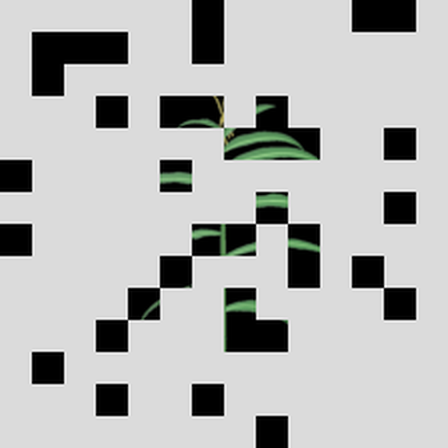
\includegraphics[width=0.4100in, height=0.4100in]{Figures/fig1b/input_rgb.png}};
\node[anchor=south west, inner sep=0] at (4.6800,1.7700) {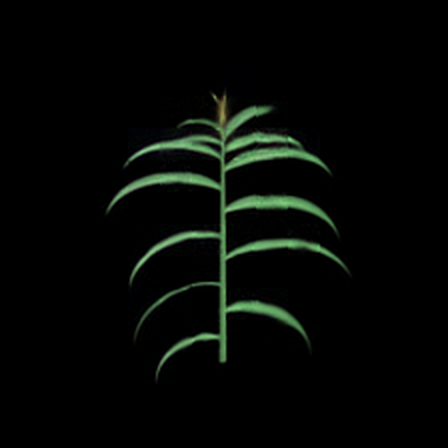
\includegraphics[width=0.4100in, height=0.4100in]{Figures/fig1b/output_rgb.png}};
\node[anchor=south west, inner sep=0] at (1.5200,1.2700) {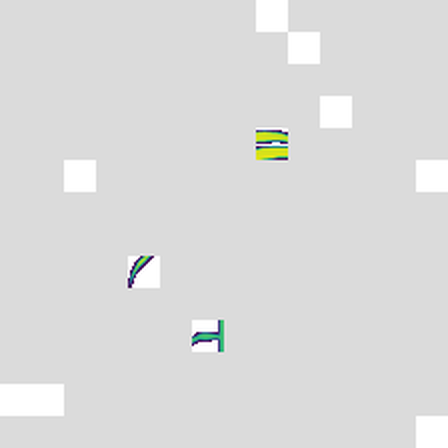
\includegraphics[width=0.4100in, height=0.4100in]{Figures/fig1b/input_depth.png}};
\node[anchor=south west, inner sep=0] at (4.6800,1.2700) {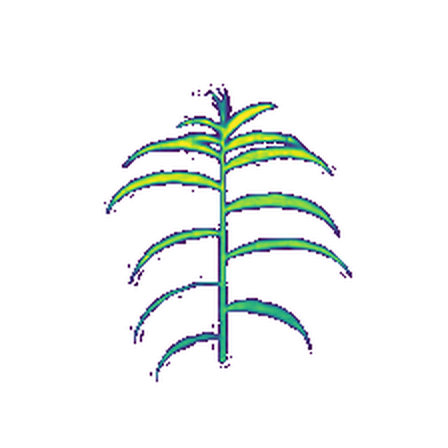
\includegraphics[width=0.4100in, height=0.4100in]{Figures/fig1b/output_depth.png}};
\node[anchor=south west, inner sep=0] at (1.5200,0.7700) {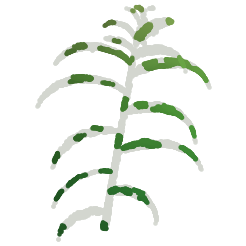
\includegraphics[width=0.4100in, height=0.4100in]{Figures/fig1b/input_pc.png}};
\node[anchor=south west, inner sep=0] at (4.6800,0.7700) {
\includegraphics[width=0.4100in, height=0.4100in]{Figures/fig1b/output_pc.png}};
\node[anchor=south west, inner sep=0] at (1.5200,0.2700) {
\includegraphics[width=0.4100in, height=0.4100in]{Figures/fig1b/input_text.png}};
\node[anchor=south west, inner sep=0] at (4.6800,0.2700) {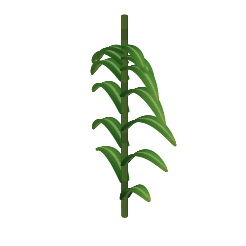
\includegraphics[width=0.4100in, height=0.4100in]{Figures/fig1b/output_text.png}};
\node[anchor=west, inner sep=0, outer sep=0, align=left, text=c1A1A1A, font={\fontsize{8.50}{10.62}\selectfont\sffamily\bfseries}] at (0.0800,2.3800) {INPUT};
\node[anchor=west, inner sep=0, outer sep=0, align=left, text=c5F5F5F, font={\fontsize{8.50}{10.62}\selectfont\sffamily}] at (0.6200,2.3800) {all four streams, 80 \% of tokens hidden};
\node[anchor=west, inner sep=0, outer sep=0, align=left, text=c1A1A1A, font={\fontsize{8.50}{10.62}\selectfont\sffamily\bfseries}] at (4.6600,2.3800) {OUTPUT};
\node[anchor=west, inner sep=0, outer sep=0, align=left, text=c5F5F5F, font={\fontsize{8.50}{10.62}\selectfont\sffamily}] at (5.3200,2.3800) {every stream rebuilt};
\draw[draw=c8C8C8C, line width=1.000pt, rounded corners=0.0800in] (2.5800,0.2500) rectangle (4.0800,2.2000);
\node[anchor=center, inner sep=0, outer sep=0, align=center, text=c1A1A1A, font={\fontsize{11.00}{13.75}\selectfont\sffamily\bfseries}] at (3.3300,1.5850) {CropCode};
\node[anchor=center, inner sep=0, outer sep=0, align=center, text=c5F5F5F, font={\fontsize{8.50}{10.62}\selectfont\sffamily}] at (3.3300,1.3250) {one model, four streams};
\node[anchor=center, inner sep=0, outer sep=0, align=center, text=c1A1A1A, font={\fontsize{8.50}{10.62}\selectfont\sffamily}] at (3.3300,1.0250) {any subset in};
\node[anchor=center, inner sep=0, outer sep=0, align=center, text=c1A1A1A, font={\fontsize{8.50}{10.62}\selectfont\sffamily}] at (3.3300,0.8250) {every stream out};
\node[anchor=west, inner sep=0, outer sep=0, align=left, text=c5F5F5F, font={\fontsize{7.00}{8.75}\selectfont\sffamily}] at (0.0800,0.0700) {held-out maize test plant · the headline model, 80 \% of all tokens hidden};
\node[anchor=east, inner sep=0, outer sep=0, align=right, text=c5E4A96, font={\fontsize{7.50}{9.38}\selectfont\sffamily}] at (6.8350,0.0700) {kilobytes  ·  editable  ·  re-renderable};
\node[anchor=east, inner sep=0, outer sep=0, align=right, text=c3F5F8F, font={\fontsize{8.50}{10.62}\selectfont\sffamily\bfseries}] at (1.4600,2.0450) {image};
\node[anchor=east, inner sep=0, outer sep=0, align=right, text=c5F5F5F, font={\fontsize{7.00}{8.75}\selectfont\sffamily}] at (1.4600,1.8850) {37 of 196 patches visible};
\draw[draw=c809EC2, line width=1.600pt, -{Triangle[length=2.80pt,width=2.80pt]}] (1.9700,1.9750) -- (2.5600,1.9500);
\draw[draw=c809EC2, line width=1.600pt, -{Triangle[length=2.80pt,width=2.80pt]}] (4.1000,1.9500) -- (4.6400,1.9750);
\node[anchor=west, inner sep=0, outer sep=0, align=left, text=c5F5F5F, font={\fontsize{8.00}{9.20}\selectfont\sffamily}] at (5.2100,1.9750) {image rebuilt};
\node[anchor=east, inner sep=0, outer sep=0, align=right, text=cA07800, font={\fontsize{8.50}{10.62}\selectfont\sffamily\bfseries}] at (1.4600,1.5450) {depth};
\node[anchor=east, inner sep=0, outer sep=0, align=right, text=c5F5F5F, font={\fontsize{7.00}{8.75}\selectfont\sffamily}] at (1.4600,1.3850) {11 of 196 patches visible};
\draw[draw=cE0B020, line width=1.600pt, -{Triangle[length=2.80pt,width=2.80pt]}] (1.9700,1.4750) -- (2.5600,1.4667);
\draw[draw=cE0B020, line width=1.600pt, -{Triangle[length=2.80pt,width=2.80pt]}] (4.1000,1.4667) -- (4.6400,1.4750);
\node[anchor=west, inner sep=0, outer sep=0, align=left, text=c5F5F5F, font={\fontsize{8.00}{9.20}\selectfont\sffamily}] at (5.2100,1.4750) {depth rebuilt};
\node[anchor=east, inner sep=0, outer sep=0, align=right, text=cA8456E, font={\fontsize{8.50}{10.62}\selectfont\sffamily\bfseries}] at (1.4600,1.0450) {point cloud};
\node[anchor=east, inner sep=0, outer sep=0, align=right, text=c5F5F5F, font={\fontsize{7.00}{8.75}\selectfont\sffamily}] at (1.4600,0.8850) {54 of 196 groups visible};
\draw[draw=cD091A7, line width=1.600pt, -{Triangle[length=2.80pt,width=2.80pt]}] (1.9700,0.9750) -- (2.5600,0.9833);
\draw[draw=cD091A7, line width=1.600pt, -{Triangle[length=2.80pt,width=2.80pt]}] (4.1000,0.9833) -- (4.6400,0.9750);
\node[anchor=west, inner sep=0, outer sep=0, align=left, text=c5F5F5F, font={\fontsize{8.00}{9.20}\selectfont\sffamily}] at (5.2100,0.9750) {cloud rebuilt\\Chamfer 0.39$\times$10\textsuperscript{$-$}\textsuperscript{3}};
\node[anchor=east, inner sep=0, outer sep=0, align=right, text=c5E4A96, font={\fontsize{8.50}{10.62}\selectfont\sffamily\bfseries}] at (1.4600,0.5450) {parameters};
\node[anchor=east, inner sep=0, outer sep=0, align=right, text=c5F5F5F, font={\fontsize{7.00}{8.75}\selectfont\sffamily}] at (1.4600,0.3850) {21 of 29 tokens visible};
\draw[draw=c9D8CC4, line width=1.600pt, -{Triangle[length=2.80pt,width=2.80pt]}] (1.9700,0.4750) -- (2.5600,0.5000);
\draw[draw=c9D8CC4, line width=1.600pt, -{Triangle[length=2.80pt,width=2.80pt]}] (4.1000,0.5000) -- (4.6400,0.4750);
\node[anchor=west, inner sep=0, outer sep=0, align=left, text=c5E4A96, font={\fontsize{8.50}{9.77}\selectfont\sffamily\bfseries}] at (5.2100,0.4750) {height 1.04 m (true 1.06)\\13 leaves (true 13)};
\end{tikzpicture}%
}%
